% Editable reconstruction; interpretation recorded in root.json.
% Shared standalone design for the editable figure reconstructions.
\documentclass[tikz,border=5pt,10pt]{standalone}
\usepackage[T1]{fontenc}
\usepackage[utf8]{inputenc}
\usepackage{newpxtext,newpxmath}
\usepackage[scaled=.94]{sourcesanspro}
\usepackage{pgfplots}
\pgfplotsset{compat=1.18}
\usetikzlibrary{arrows.meta,calc,positioning,decorations.pathreplacing,
  decorations.markings,patterns,matrix,shapes.geometric,fit,backgrounds,
  intersections,angles,quotes}
\definecolor{ink}{HTML}{203746}
\definecolor{accent}{HTML}{146C78}
\definecolor{muted}{HTML}{667780}
\definecolor{signalred}{HTML}{B94B44}
\color{ink}
\tikzset{>=Latex,line width=.8pt,
  every node/.style={font=\small},
  axis/.style={->,draw=muted,line width=.5pt},
  guide/.style={draw=muted,dashed,line width=.45pt},
  curve/.style={draw=accent,line width=1pt},
  marker/.style={circle,fill=accent,inner sep=1.5pt},
  labelbox/.style={fill=white,inner sep=2pt}}

\begin{document}
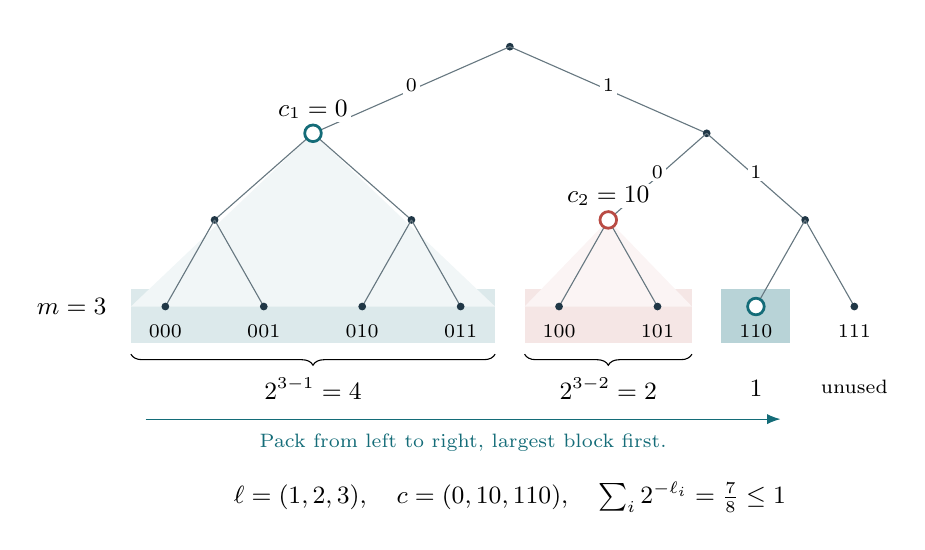
\begin{tikzpicture}[x=1.25cm,y=1.1cm]
\fill[accent!15] (-3.85,-3.42) rectangle (-.15,-2.8);
\fill[signalred!14] (.15,-3.42) rectangle (1.85,-2.8);
\fill[accent!30] (2.15,-3.42) rectangle (2.85,-2.8);
% The tinted regions identify the disjoint descendant subtrees.
\fill[accent!6] (-2,-1)--(-3.85,-3)--(-.15,-3)--cycle;
\fill[signalred!6] (1,-2)--(.15,-3)--(1.85,-3)--cycle;
\fill[ink] (0.000,0) circle(1.4pt);
\draw[muted] (0.000,0)--(-2.000,-1);
\fill[ink] (-2.000,-1) circle(1.4pt);
\draw[muted] (0.000,0)--(2.000,-1);
\fill[ink] (2.000,-1) circle(1.4pt);
\draw[muted] (-2.000,-1)--(-3.000,-2);
\fill[ink] (-3.000,-2) circle(1.4pt);
\draw[muted] (-2.000,-1)--(-1.000,-2);
\fill[ink] (-1.000,-2) circle(1.4pt);
\draw[muted] (2.000,-1)--(1.000,-2);
\fill[ink] (1.000,-2) circle(1.4pt);
\draw[muted] (2.000,-1)--(3.000,-2);
\fill[ink] (3.000,-2) circle(1.4pt);
\draw[muted] (-3.000,-2)--(-3.500,-3);
\fill[ink] (-3.500,-3) circle(1.4pt);
\node[below=3pt,font=\scriptsize] at (-3.500,-3) {000};
\draw[muted] (-3.000,-2)--(-2.500,-3);
\fill[ink] (-2.500,-3) circle(1.4pt);
\node[below=3pt,font=\scriptsize] at (-2.500,-3) {001};
\draw[muted] (-1.000,-2)--(-1.500,-3);
\fill[ink] (-1.500,-3) circle(1.4pt);
\node[below=3pt,font=\scriptsize] at (-1.500,-3) {010};
\draw[muted] (-1.000,-2)--(-0.500,-3);
\fill[ink] (-0.500,-3) circle(1.4pt);
\node[below=3pt,font=\scriptsize] at (-0.500,-3) {011};
\draw[muted] (1.000,-2)--(0.500,-3);
\fill[ink] (0.500,-3) circle(1.4pt);
\node[below=3pt,font=\scriptsize] at (0.500,-3) {100};
\draw[muted] (1.000,-2)--(1.500,-3);
\fill[ink] (1.500,-3) circle(1.4pt);
\node[below=3pt,font=\scriptsize] at (1.500,-3) {101};
\draw[muted] (3.000,-2)--(2.500,-3);
\fill[ink] (2.500,-3) circle(1.4pt);
\node[below=3pt,font=\scriptsize] at (2.500,-3) {110};
\draw[muted] (3.000,-2)--(3.500,-3);
\fill[ink] (3.500,-3) circle(1.4pt);
\node[below=3pt,font=\scriptsize] at (3.500,-3) {111};
\draw[accent,fill=white,line width=1pt] (-2,-1) circle(3pt);
\node[above=4pt,fill=white,inner sep=1pt] at (-2,-1) {$c_1=0$};
\draw[signalred,fill=white,line width=1pt] (1,-2) circle(3pt);
\node[above=4pt,fill=white,inner sep=1pt] at (1,-2) {$c_2=10$};
\draw[accent,fill=white,line width=1pt] (2.5,-3) circle(3pt);
\node[font=\scriptsize,fill=white,inner sep=1pt] at (-1,-.45) {$0$};
\node[font=\scriptsize,fill=white,inner sep=1pt] at (1,-.45) {$1$};
\node[font=\scriptsize,fill=white,inner sep=1pt] at (1.5,-1.45) {$0$};
\node[font=\scriptsize,fill=white,inner sep=1pt] at (2.5,-1.45) {$1$};
\node[above] at (0,0) {$\varnothing$};\node[left] at (-4,-3) {$m=3$};
\draw[decorate,decoration={brace,mirror,amplitude=4pt}] (-3.85,-3.55)--(-.15,-3.55) node[midway,below=5pt] {$2^{3-1}=4$};
\draw[decorate,decoration={brace,mirror,amplitude=4pt}] (.15,-3.55)--(1.85,-3.55) node[midway,below=5pt] {$2^{3-2}=2$};
\node[below=6pt] at (2.5,-3.55) {$1$};
\node[below=6pt,font=\scriptsize] at (3.5,-3.55) {unused};
\draw[->,accent] (-3.7,-4.3)--(2.75,-4.3) node[midway,below=2pt,font=\scriptsize] {Pack from left to right, largest block first.};
\node at (0,-5.2) {$\ell=(1,2,3),\quad c=(0,10,110),\quad\sum_i2^{-\ell_i}=\frac78\leq1$};
\end{tikzpicture}
\end{document}
